\documentclass[aspectratio=169]{../latex_main/tntbeamer}  % you can pass all options of the beamer class, e.g., 'handout' or 'aspectratio=43'
\usepackage{dsfont}
\usepackage{bm}
\usepackage[english]{babel}
\usepackage[T1]{fontenc}
%\usepackage[utf8]{inputenc}
\usepackage{graphicx}
\graphicspath{ {./figures/} }
\usepackage{algorithm}
\usepackage[ruled,vlined,algo2e,linesnumbered]{algorithm2e}
\usepackage{hyperref}
\usepackage{booktabs}
\usepackage{mathtools}

\usepackage{amsmath,amssymb}

\DeclareMathOperator*{\argmax}{arg\,max}
\DeclareMathOperator*{\argmin}{arg\,min}

\usepackage{amsbsy}
\newcommand{\vect}[1]{\bm{#1}}
%\newcommand{\vect}[1]{\boldsymbol{#1}}

\usepackage{pgfplots}
\pgfplotsset{compat=1.16}
\usepackage{tikz}
\usetikzlibrary{trees} 
\usetikzlibrary{shapes.geometric}
\usetikzlibrary{positioning,shapes,shadows,arrows,calc,mindmap}
\usetikzlibrary{positioning,fadings,through}
\usetikzlibrary{decorations.pathreplacing}
\usetikzlibrary{intersections}
\pgfdeclarelayer{background}
\pgfdeclarelayer{foreground}
\pgfsetlayers{background,main,foreground}
\tikzstyle{activity}=[rectangle, draw=black, rounded corners, text centered, text width=8em]
\tikzstyle{data}=[rectangle, draw=black, text centered, text width=8em]
\tikzstyle{myarrow}=[->, thick, draw=black]

% Define the layers to draw the diagram
\pgfdeclarelayer{background}
\pgfdeclarelayer{foreground}
\pgfsetlayers{background,main,foreground}

% Requires XeLaTeX or LuaLaTeX
%\usepackage{unicode-math}

\usepackage{fontspec}
%\setsansfont{Arial}
\setsansfont{RotisSansSerifStd}[ 
Path=../latex_main/fonts/,
Extension = .otf,
UprightFont = *-Regular,  % or *-Light
BoldFont = *-ExtraBold,  % or *-Bold
ItalicFont = *-Italic
]
\setmonofont{Cascadia Mono}[
Scale=0.8
]

% scale factor adapted; mathrm font added (Benjamin Spitschan @TNT, 2021-06-01)
%\setmathfont[Scale=1.05]{Libertinus Math}
%\setmathrm[Scale=1.05]{Libertinus Math}

% other available math fonts are (not exhaustive)
% Latin Modern Math
% XITS Math
% Libertinus Math
% Asana Math
% Fira Math
% TeX Gyre Pagella Math
% TeX Gyre Bonum Math
% TeX Gyre Schola Math
% TeX Gyre Termes Math

% Literature References
\newcommand{\lit}[2]{\href{#2}{\footnotesize\color{black!60}[#1]}}

%%% Beamer Customization
%----------------------------------------------------------------------
% (Don't) Show sections in frame header. Options: 'sections', 'sections light', empty
\setbeamertemplate{headline}{empty}

% Add header logo for normal frames
\setheaderimage{
	% 
\includegraphics[height=\logoheight]{figures/TNT_darkv4.pdf}
	
\includegraphics[height=\logoheight]{../latex_main/figures/luh_logo_rgb_0_80_155.pdf}
	% 
\includegraphics[height=\logoheight]{figures/logo_tntluh.pdf}
}

% Header logo for title page
\settitleheaderimage{
	% 
\includegraphics[height=\logoheight]{figures/TNT_darkv4.pdf}
	
\includegraphics[height=\logoheight]{../latex_main/figures/luh_logo_rgb_0_80_155.pdf}
	% 
\includegraphics[height=\logoheight]{figures/logo_tntluh.pdf}
}

% Title page: tntdefault 
\setbeamertemplate{title page}[tntdefault]  % or luhstyle
% Add optional title image here
%\addtitlepageimagedefault{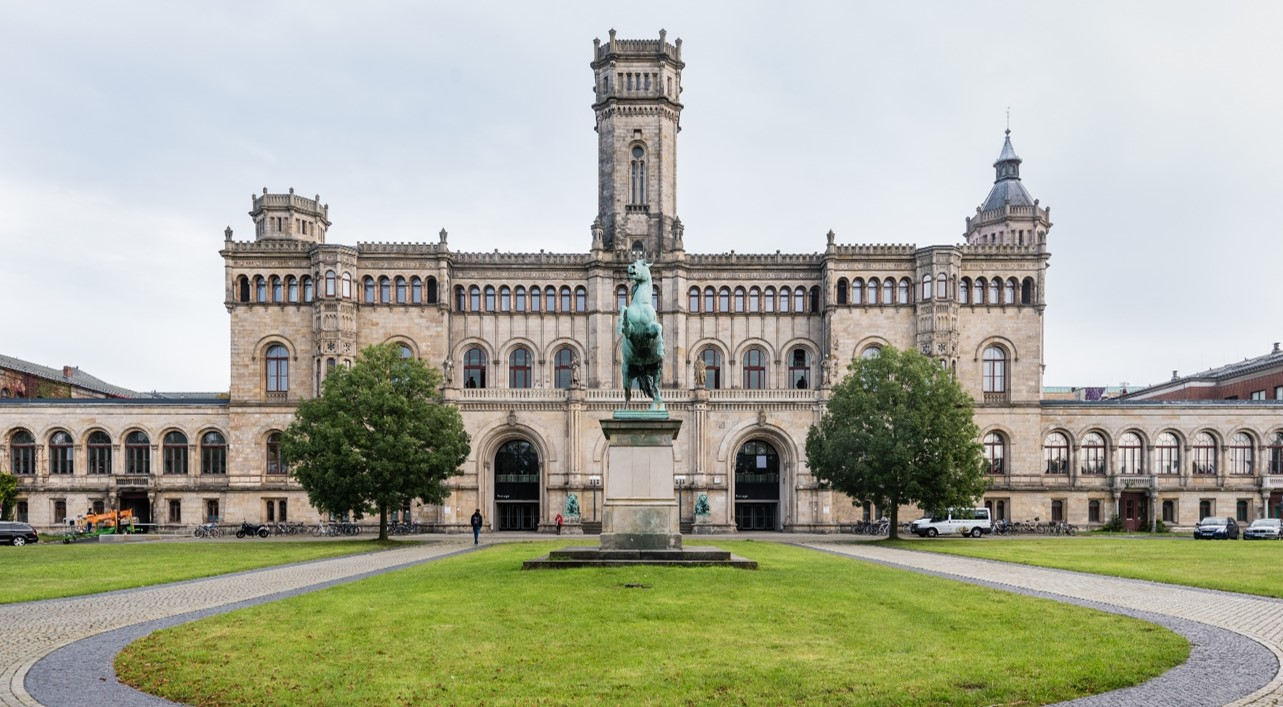
\includegraphics[width=0.65\textwidth]{figures/luh_default_presentation_title_image.jpg}}

% Title page: luhstyle
% \setbeamertemplate{title page}[luhstyle]
% % Add optional title image here
% \addtitlepageimage{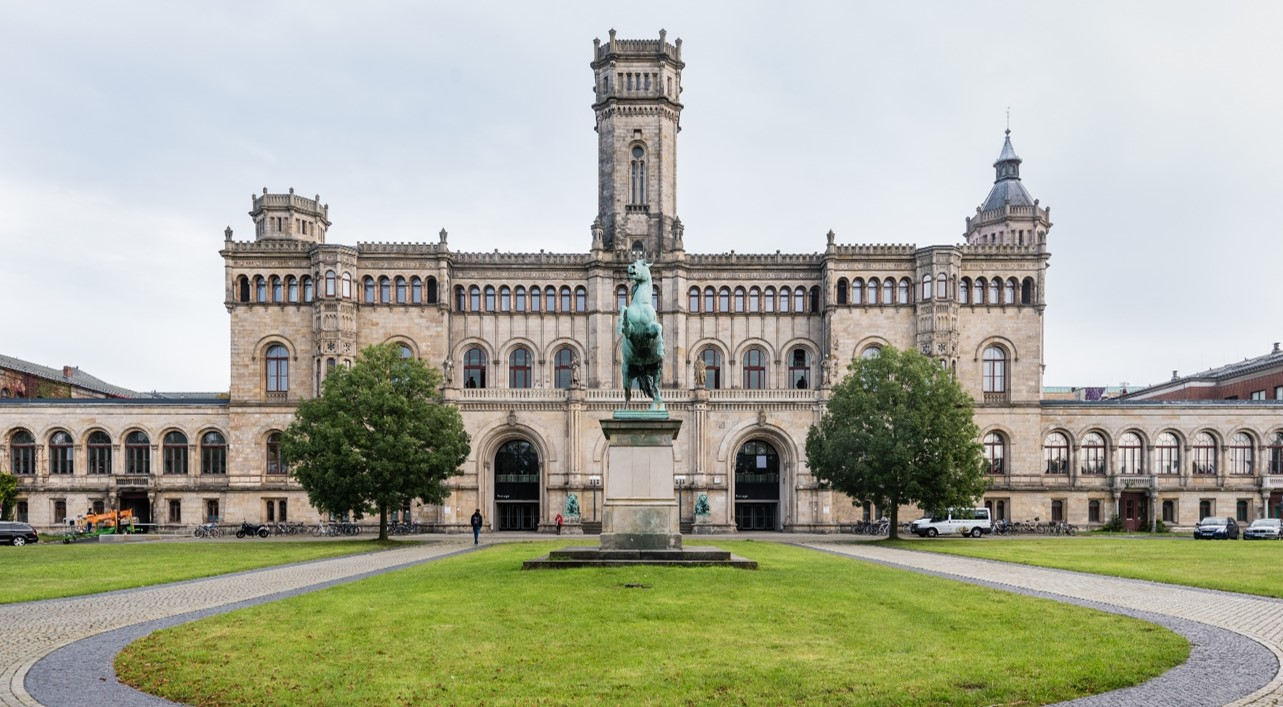
\includegraphics[width=0.75\textwidth]{figures/luh_default_presentation_title_image.jpg}}

\author[Abedjan \& Lindauer]{Ziawasch Abedjan \& Marius Lindauer\\[1em]
	
\includegraphics[height=\logoheight]{../latex_main/figures/luh_logo_rgb_0_80_155.pdf}\qquad
	
\includegraphics[height=\logoheight]{../latex_main/figures/DBIS_Kurzlogo.png}\qquad

\includegraphics[height=\logoheight]{../latex_main/figures/TNT_darkv4}\qquad

\includegraphics[height=\logoheight]{../latex_main/figures/L3S.jpg}	}
\date{Summer Term 2022; \hspace{0.5em} {
\includegraphics[height=1.5em]{../latex_main/figures/Cc-by-nc-sa_icon.svg.png}}; based on \href{https://ds100.org/fa21/}{[DS100]}
}


%%% Custom Packages
%----------------------------------------------------------------------
% Create dummy content
\usepackage{blindtext}

% Adds a frame with the current page layout. Just call \layout inside of a frame.
\usepackage{layout}


%%% Macros
%\renewcommand{\vec}[1]{\mathbf{#1}}
% \usepackage{bm}
%\let\vecb\bm

\title[Introduction]{DS: Conclusion}
\subtitle{What did you learn in this class?}

\graphicspath{ {./figure/} }
%\institute{}


\begin{document}
	
	\maketitle
	\begin{frame}{What were we supposed to teach you?}
	    \begin{columns}
	      \begin{column}{.3\textwidth}
	            \begin{center}
	                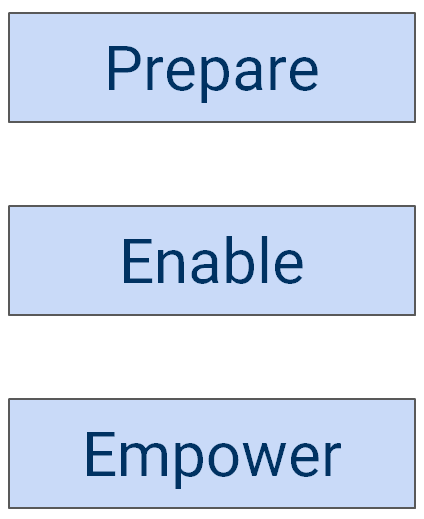
\includegraphics[scale=.4]{Bild1}
	            \end{center}
	                
	       \end{column}
	       
	       \begin{column}{.7\textwidth}
	           \\\bigskip
	           Prepare students for advanced Berkeley courses in data management, machine learning, and statistics, by providing the necessary foundation and context.\\
	           \bigskip
	           \smallskip
	           Enable students to start careers as data scientists by providing experience working with real-world data, tools, and techniques.\\
	           \bigskip
	           \bigskip
	           \medskip
	           \medskip
	           Empower students to apply computational and inferential thinking to address real-world problems.
	       \end{column}
        \end{columns}

	\end{frame}
	
	
	 \begin{frame}{Note}
	     \begin{itemize}
	         \item The following is a high-level overview of what we covered.
	         \item You may find this useful in organizing your studying.
	         \item But this is not comprehensive!
	     \end{itemize}
	 \end{frame}
	 
	 
	 
	 \begin{frame}{Data sampling and probability}
	     \begin{itemize}
	         \item Populations, samples, and sampling frames (Lecture 2).
	         \begin{itemize}
	             \item Sources of bias in sampling.
	             \item Types of samples (random samples vs. convenience samples, quota samples).
	             \item Benefits of random sampling.
	             \begin{itemize}
	                 \item Larger samples are not necessarily better.
	                 \item Large biased samples can make things worse.
	             \end{itemize}
	             \item Sampling with and without replacement.
	             \item Binomial and multinomial probabilities.
	         \end{itemize}
	         \item Estimation and statistical bias (Lecture 3).
	         \begin{itemize}
	             \item Introduction to random variables
	             \item Expectation and its properties (e.g. linearity of expectation).
	             \item What an estimator is, and how we can calculate its bias.
	         \end{itemize}
	     \end{itemize}
	 \end{frame}
	 
	 
	 \begin{frame}{Pandas and data cleaning}
	     \begin{itemize}
	         \item pandas as a means of working with tabular data in Python (Lectures 4, 5).
	         \begin{itemize}
	             \item Series, DataFrames, and indexes.
	             \item .loc and .iloc.
	             \item Filtering, merging, grouping, pivoting, etc.
	         \end{itemize}
	         \item Data cleaning and exploratory data analysis (Lecture 6).
	         \begin{itemize}
	             \item Structure, granularity, scope, temporality, faithfulness.
	             \item Handling missing values.
	         \end{itemize}
	     \end{itemize}
	     \hfill
	     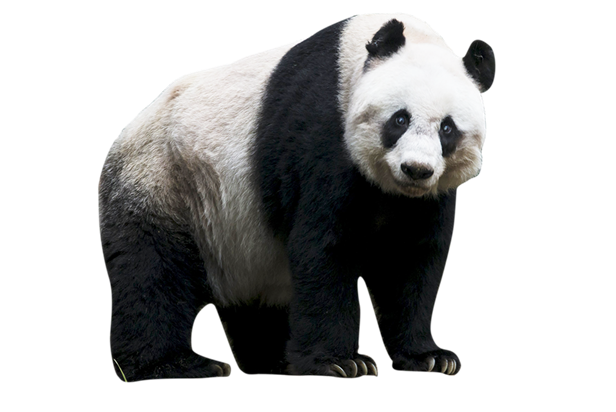
\includegraphics[scale=.5]{Bild2}
	 \end{frame}
	 
	 
	 
	 
	 \begin{frame}{Regex and SQL}
	     \begin{itemize}
	         \item Regular expressions as a means of identifying and extracting patterns in text (Lecture 7).
	         \begin{itemize}
	             \item Python string expressions.
	             \item regex101.com is your friend!
	         \end{itemize}
	         \item SQL as a means of querying large databases (Lecture 8).
	         \begin{itemize}
	             \item Primary keys and foreign keys.
	             \item Types of joins.
	         \end{itemize}
	     \end{itemize}
	     \\\bigskip
	     
\includegraphics[scale=.4]{Bild3}
	 \end{frame}
	 
	 
	 
	 \begin{frame}{Visualization}
	    \begin{columns}
	      \begin{column}{.5\textwidth}
	            \begin{itemize}
	                \item Visualization (Lectures 9, 10).
	                \begin{itemize}
	                    \item Encodings and distributions.
	                    \item When and how: bar plots, rug plots, histograms, density curves, box plots, violin plots, scatter plots, hex plots, contour plots.
	                    \item Describing distributions in statistical terms (tails, skew, modes, outliers).
	                    \item Principles of scale, conditioning, perception, and context.
	                    \item Kernel density estimation.
	                    \item Transformations.
	                \end{itemize}
	            \end{itemize}
	                
	       \end{column}
	       
	       \begin{column}{.4\textwidth}
	          \begin{center}
	              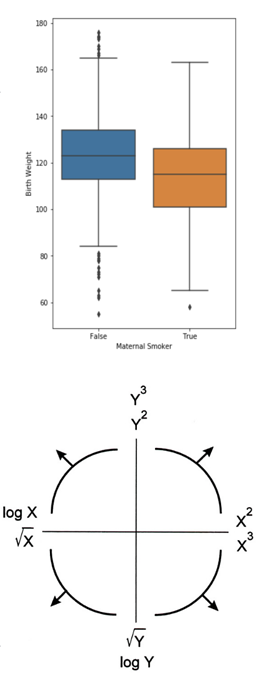
\includegraphics[scale=.33]{Bild4}
	          \end{center}
	       \end{column}
        \end{columns}

	\end{frame}
	
	
	\begin{frame}{Modeling and linear regression}
	            \begin{itemize}
	                \item The modeling “recipe” (Lecture 11).
	                \begin{itemize}
	                    \item Encodings and distributions.Choose a model (e.g. constant model, linear regression, logistic regression).
	                    \item Choose a loss function (e.g. squared loss, absolute loss, cross-entropy loss).
	                    \item Determine optimal parameters that minimize average loss (i.e. empirical risk) on training data.
	                \end{itemize}
	                \item  Simple linear regression (Lecture 12).  
	                \begin{centering} 
                        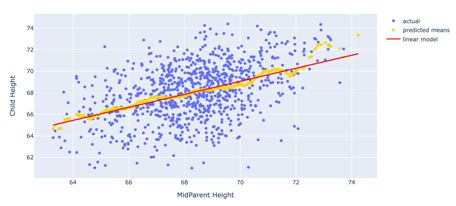
\includegraphics[scale=.3]{Bild5}
                    \end{centering} 
	                \begin{itemize}
	                    \item Correlation coefficient r.
	                    \item Finding optimal parameters by hand with calculus.
	                    \item RMSE, Multiple $R^2$.
	                \end{itemize}
	                \item  Ordinary least squares (Lecture 13).
	                \begin{itemize}
	                    \item Regression: given features, compute a real-valued prediction for each observation.
	                    \item Design matrices, residuals, orthogonality.
	                    \item Normal equation.
	                \end{itemize}
	            \end{itemize}
	            
	              
	\end{frame}
	
	
	
	
	\begin{frame}{Feature engineering, bias-variance tradeoff}
	          \begin{columns}
	            \begin{column}{.7\textwidth}

	            \begin{itemize}
	                \item Feature engineering: how do we model non-numeric and non-linear relationships, using linear models? (Lecture 14)
	                \begin{itemize}
	                    \item Categorical: one-hot encoding, bag-of-words, n-gram.
	                    \item Polynomial features.
	                    \item Overfitting to training data.
	                \end{itemize}
	                \item  Bias-Variance tradeoff (Lecture 16).
	                \begin{itemize}
	                    \item What are the underlying assumptions of randomness when modeling? (true model, random noise, etc.)
	                    \item As we increase complexity, what happens to model bias? Model variance?
	                    \item Model risk and its decomposition.
	                \end{itemize}
	            \end{itemize}
	            \end{column}
	            
	            
	            \begin{column}{.3\textwidth}
	                      \begin{center}
	                          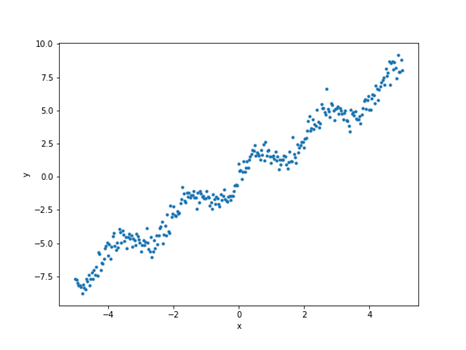
\includegraphics[scale=.65]{Bild6}
	                      \end{center} 
	            \end{column}
	       \end{columns}
	\end{frame}
	
	
	\begin{frame}{Context in modeling}
	          \begin{columns}
	            \begin{column}{.6\textwidth}
	            \vspace{.75cm}
	            \begin{itemize}
	                \item CCAO case study (Lecture 15)
	                \begin{itemize}
	                    \item How the models we build can have real-world consequences on real-life people
	                    \item Is accuracy all that matters?
	                    \item Overfitting to training data.
	                    \item Limits of data analysis
	                    \item Thinking about the context behind the choices made when collecting data, choosing models, etc.
	                \end{itemize}
	            \end{itemize}
	            \begin{center}
	                
\includegraphics[scale=.5]{Bild8}
	            \end{center}
	            \end{column}
	            
	            
	            \begin{column}{.4\textwidth}
	                      \begin{center}
	                          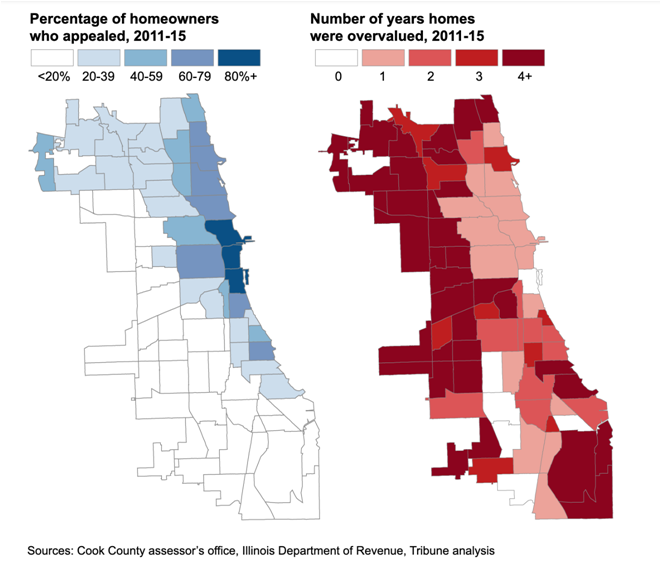
\includegraphics[scale=.55]{Bild7}
	                      \end{center} 
	            \end{column}
	       \end{columns}
	\end{frame}
	
	
	
	\begin{frame}{Regularization and cross-validation}
	          \begin{columns}
	            \begin{column}{.6\textwidth}
	           % \vspace{.75cm}
	            \begin{itemize}
	                \item Cross-validation as a means of selecting hyperparameters and/or sets of features (Lecture 17).
	                \begin{itemize}
	                    \item Train-test splits, and why they’re necessary.
	                    \item Cross-validation as a means of estimating model performance on testing data using just training data. 
	                \end{itemize}
	                \item Regularization as a means of controlling model complexity (Lecture 17).
	                \begin{itemize}
	                    \item Penalties on the norm of parameter vectors.
	                    \item Ridge and LASSO.
	                    \item Effects of the regularization hyperparameter on model complexity.
	                \end{itemize}
	            \end{itemize}
	            \end{column}
	            
	            
	            \begin{column}{.4\textwidth}
	                        \vspace{1.5cm}
	                      \begin{center}
	                          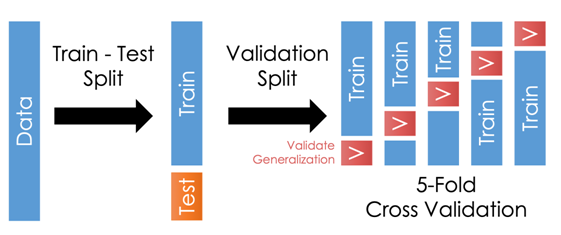
\includegraphics[scale=.55]{Bild9}
	                      \end{center} 
	            \end{column}
	       \end{columns}
	\end{frame}
	
	
	
	\begin{frame}{Generalization}
	    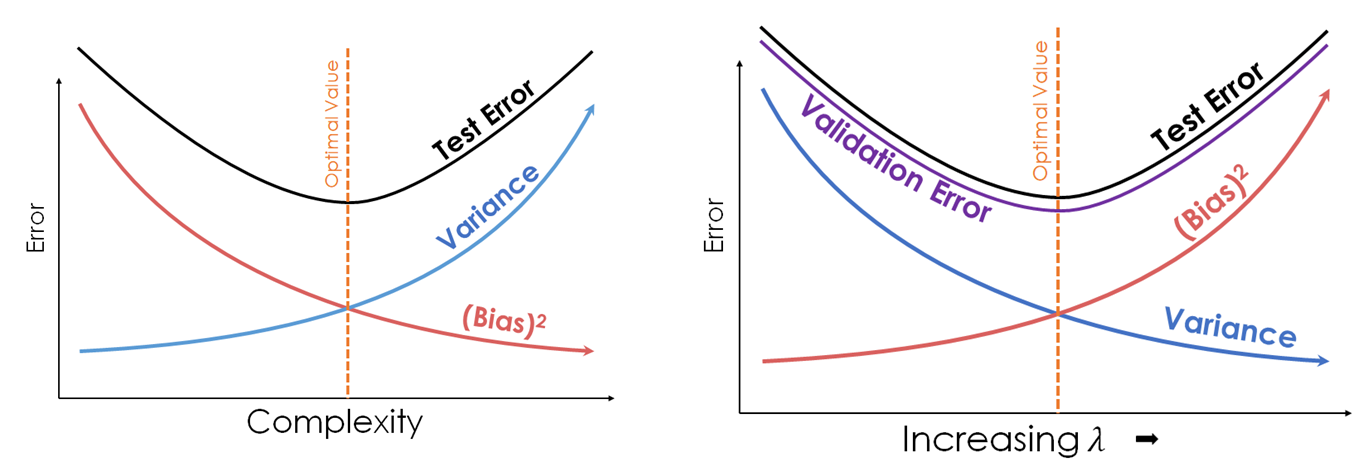
\includegraphics[scale=.4]{Bild10}\\
	    Our ultimate goal is to build models that generalize well to unseen data. The bias-variance tradeoff, training error, testing error, and cross-validation error all describe how well our model generalizes.

	\end{frame}
	
	
	
	\begin{frame}{Gradient descent}
	          \begin{columns}
	            \begin{column}{.6\textwidth}
	           % \vspace{.75cm}
	            \begin{itemize}
	                \item Gradient descent as a means of numerically minimizing functions (Lecture 18).
	                \begin{itemize}
	                    \item For our purposes, used to minimize average loss across a dataset.
	                    \item Convexity.
	                    \begin{itemize}
	                        \item If our loss function is not convex for our model, gradient descent may get stuck in a local minima.
	                    \end{itemize}
	                    \item Learning rates.
	                    \begin{itemize}
	                        \item The size of the steps we take can affect whether or not we converge.
	                    \end{itemize}
	                    \item Stochastic gradient descent.
	                \end{itemize}
	            \end{itemize}
	            \end{column}
	            
	            
	            \begin{column}{.4\textwidth}
	                      \begin{center}
	                          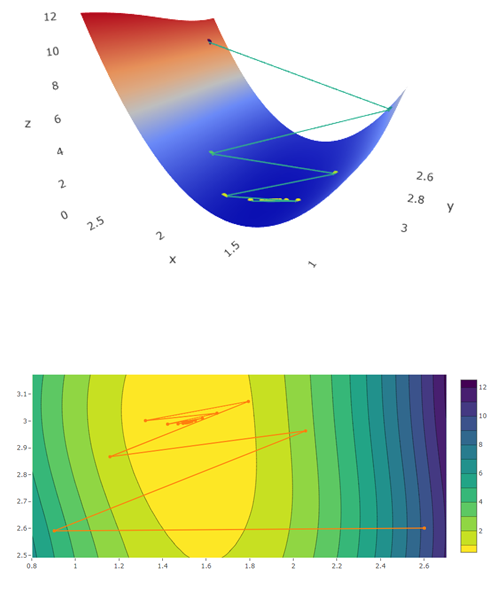
\includegraphics[scale=.38]{Bild11}
	                      \end{center} 
	            \end{column}
	       \end{columns}
	\end{frame}
	
	
	
	\begin{frame}{Logistic regression and classification}
	          \begin{columns}
	            \begin{column}{.6\textwidth}
	           % \vspace{.75cm}
	            \begin{itemize}
	                \item Classification: given features, compute a discrete label for each observation.
	                \item Logistic regression as a model of probabilities (Lecture 19).
	                \begin{itemize}
	                    \item Linearity of log-odds.
	                    \item The logistic function and its properties.
	                    \item Cross-entropy loss vs. squared loss for logistic regression.
	                \end{itemize}
	                \item Classification and classifier evaluation (Lecture 20).
	                \begin{itemize}
	                    \item Thresholding and decision boundaries.
	                    \item Linear separability, and the need for regularization.
	                    \item Accuracy, precision, and recall. Confusion matrices.
	                    \item PR curves, ROC curves, and AUC.
	                \end{itemize}
	            \end{itemize}
	            \end{column}
	            
	            
	            \begin{column}{.4\textwidth}
	                      \begin{center}
	                          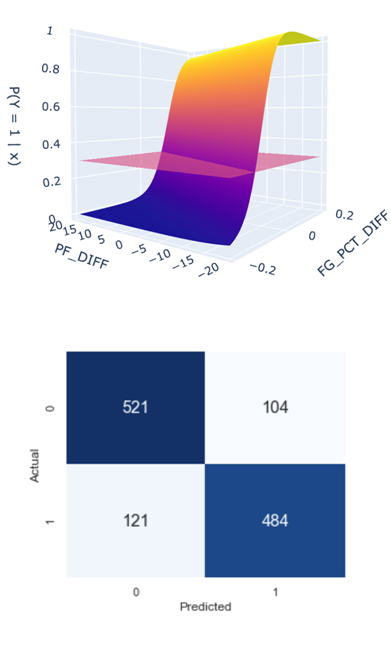
\includegraphics[scale=.35]{Bild12}
	                      \end{center} 
	            \end{column}
	       \end{columns}
	\end{frame}
	
	
	
	\begin{frame}{Decision trees, model inference, PCA, clustering}
	    \begin{itemize}
	        \item Decision trees and random forests: an alternative to regression and classification (Lecture 21).
	        \item Model inference: using statistical tools to interpret our model’s parameters (Lecture 22).
	        \begin{itemize}
	            \item Parameters, estimators, the bootstrap, and confidence intervals.
	            \item Multicollinearity.
	        \end{itemize}
	        \item Unsupervised learning: instead of trying to learn the relationship between features and a response variable, we instead try and learn the pattern amongst the data itself.
	        \begin{itemize}
	            \item PCA (Lecture 23): How can we extract meaningful combinations of features from our high-dimensional data? What are “orthogonal basis vectors”?
	            \item Clustering (Lectures 24 and 25): How can we segment our data into “groups” that are similar to one another?
	            \begin{itemize}
	                \item  Graphs, a different approach of representing data
	            \end{itemize}
	        \end{itemize}
	    \end{itemize}
	\end{frame}
	
	
	\begin{frame}{Labs}
	    \begin{itemize}
	        \item Lab 1: Python programming and plotting.
	        \item Lab 2: Introduction to pandas.
	        \item Lab 3: Data cleaning, EDA, and basic visualization.
	        \item Lab 4: SQL.
	        \item Lab 5: More visualization – transformations, kernel density estimation.
	        \item Lab 6: Modeling and loss functions, focusing on the constant model.
	        \item Lab 7: Finding optimal model coefficients for simple linear regression in several different ways, and an introduction to multiple regression.
	        \item Lab 8: Feature engineering, and regression in scikit-learn.
	        \item Lab 9: Implementing cross-validation for feature selection.
	        \item Lab 10: An introduction to logistic regression.
	        \item Lab 11: Multi-class logistic regression, decision trees, and random forests.
	        \item Lab 12: PCA.
	        \item Lab 13: Clustering.
	    \end{itemize}
	\end{frame}
	
	
	\begin{frame}{Homeworks}
	    \begin{itemize}
	        \item Homework 1: Calculus, linear algebra, and Data 8 prerequisite review.
	        \item Homework 2: A study of sampling error and bias on 2016 presidential election polling data.
	        \item Homework 3: Data cleaning and EDA on San Francisco restaurant food safety scores.
	        \item Homework 4: Text analysis on Tweets from AOC, Elon Musk, and CR7.
	        \item Homework 5: EDA and Visualization of San Francisco bike sharing data.
	        \item Homework 6: Math behind linear regression.
	        \item Homework 7: Feature engineering on housing data from Cook County, IL.
	        \item Homework 8: Linear modeling, and contextual questions on housing data from Cook County, IL.
	        \item Homework 9: Gradient descent.
	        \item Homework 10: EDA on ham/spam emails. 
	        \item Homework 11: Classification and prediction on ham/spam emails. 
	        \item Homework 12: Using PCA to study midterm data and historical election data.
	    \end{itemize}
	\end{frame}
	
	
	\begin{frame}{Data science lifecycle}
	    \begin{columns}
	      \begin{column}{.5\textwidth}
	              \begin{center}
	                  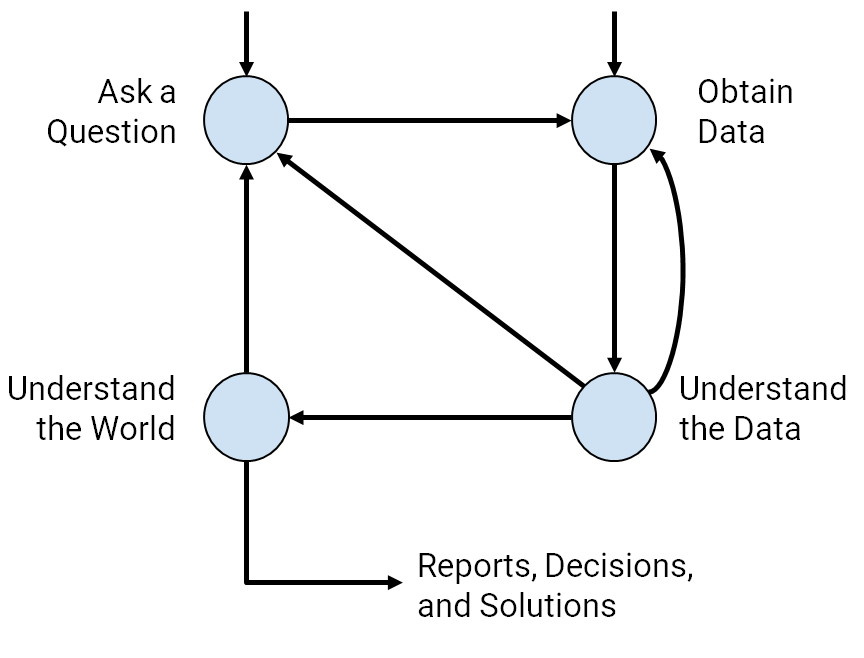
\includegraphics[scale=.35]{Bild13}
	              \end{center}
	      \end{column}
	      
	      
	      \begin{column}{.5\textwidth}
	              \vspace{2cm}
	              \\The data science lifecycle is a high-level description of the data science workflow.\\
                  \bigskip
                  Note the two distinct entry points!
	      \end{column}
	    \end{columns}
	\end{frame}
	
	
	
	\begin{frame}{Useful libraries and programming tools}
	    \centering
	    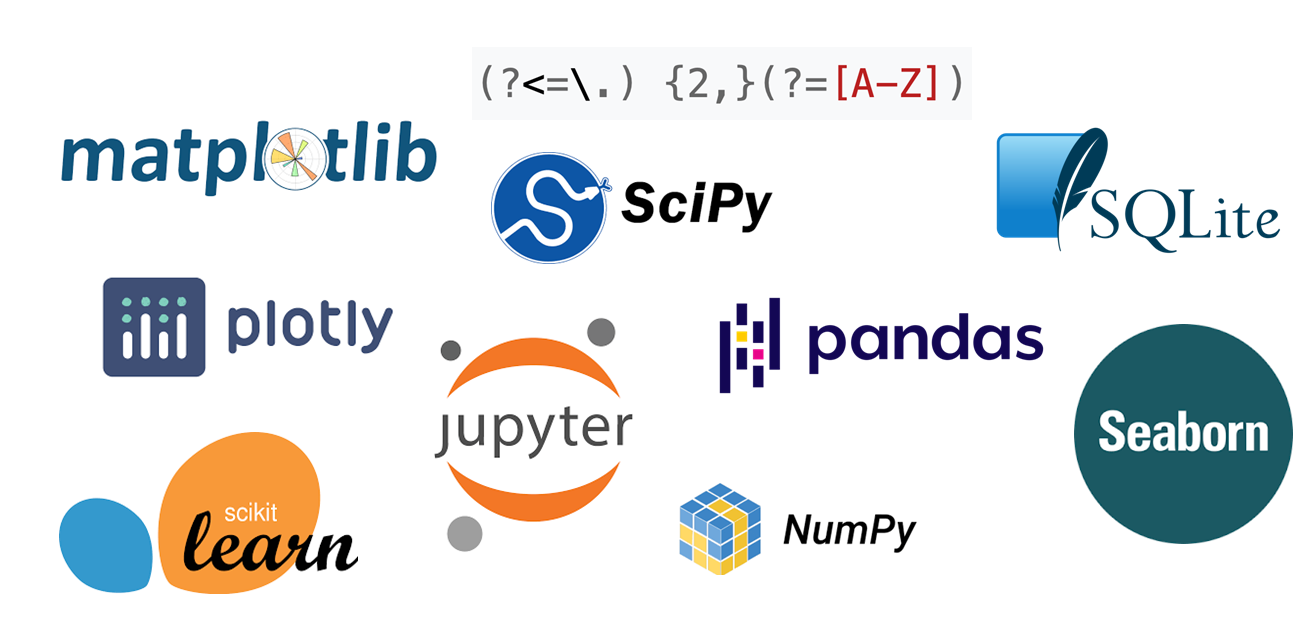
\includegraphics[scale=.35]{Bild14}
	\end{frame}
\end{document}